\subsubsection{2.5. Mạng noron đồ thị (GNN)}
\indent\indent Mạng noron đồ thị (GNN) \cite{hamilton2020graph} là một mô hình học sâu được thiết kế để xử lý dữ liệu có cấu trúc đồ thị. Mục tiêu cốt lõi của GNN là học một vector biểu diễn (embedding) cho mỗi đỉnh, cạnh hoặc toàn bộ đồ thị, sao cho vector này bảo toàn được cả đặc trưng tại các đỉnh và thông tin cấu trúc của đồ thị đó.\vspace{0.3cm}

\begin{figure}[H]
    \centering
    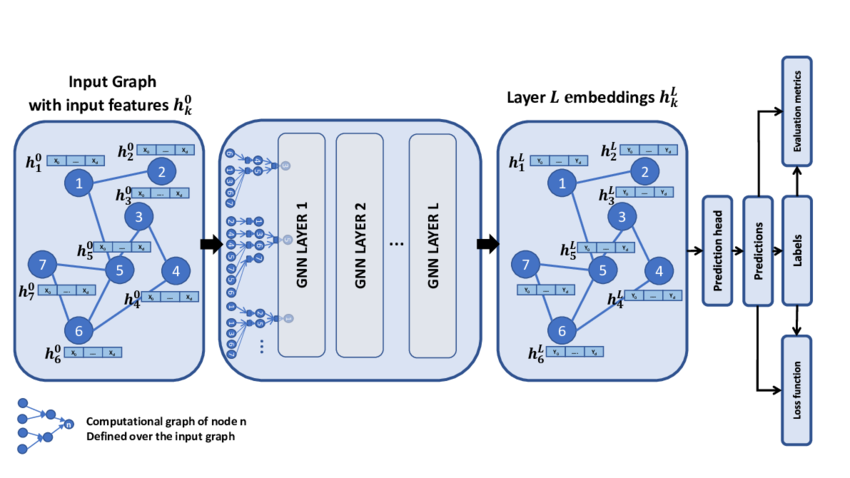
\includegraphics[width=0.8\linewidth]{images/part-02/chap-01/GNN.png}
    \vspace{0.5cm}
    \caption{Minh hoạ kiến trúc cơ bản của GNN}
    \label{fig:GNN}
\end{figure}

Cơ chế hoạt động nền tảng của hầu hết các GNN hiện đại là truyền thông điệp (Message Passing). Tại mỗi tầng $k$, vector đặc trưng của đỉnh $v$ được cập nhật bằng cách tổng hợp thông tin từ các đỉnh hàng xóm $N(v)$:
\[
    h_v^{(k)} = \text{UPDATE}^{(k)} \left( h_v^{(k-1)}, \text{AGGREGATE}^{(k)} \left( \{ h_u^{(k-1)} | u \in N(v) \} \right) \right)
\]
Trong đó $h_v^{(k)}$ là hidden state của đỉnh $v$ tại tầng $k$, hàm AGGREGATE có nhiệm vụ gom thông tin từ hàng xóm, và hàm UPDATE kết hợp thông tin đó với trạng thái hiện tại của đỉnh.\vspace{0.3cm}

Có rất nhiều phiên bản cụ thể được triển khai từ GNN, trong đó nổi bật nhất phải kể đến Graph Attention Network (GAT). Kiến trúc này được giới thiệu bởi Veličković và cộng sự \cite{veličković2018graphattentionnetworks}, họ đề xuất cơ chế self-attention để học trọng số cho các cạnh. Điều này cho phép mô hình tập trung vào các hàng xóm quan trọng nhất đối với đỉnh đang xét.\vspace{0.3cm}

\begin{figure}[H]
    \centering
    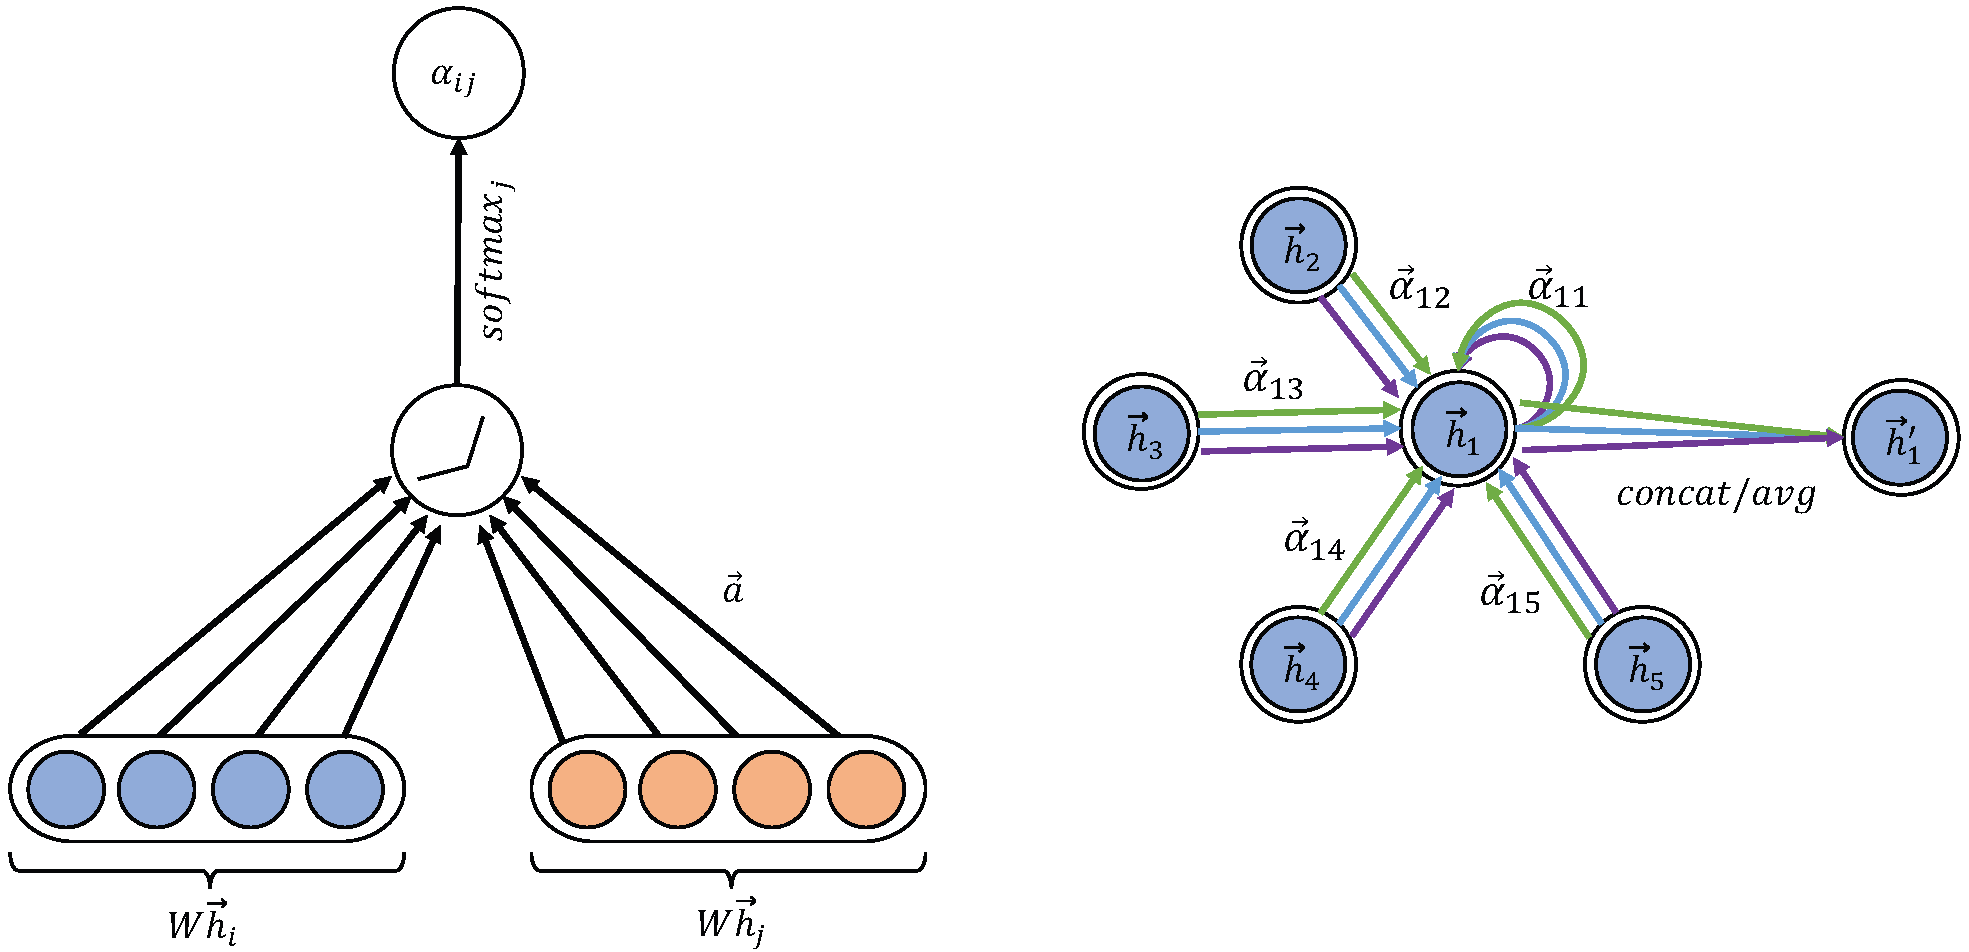
\includegraphics[width=0.8\linewidth]{images/part-02/chap-01/GAT.png}
    \vspace{0.5cm}
    \caption{Minh hoạ kiến trúc cơ bản của GAT}
    \label{fig:GAT}
\end{figure}

Cơ chế Attention trong GAT được thực hiện như sau:
\begin{itemize}[label={--}, itemsep=1pt]
    \item Đầu tiên, hệ số chú ý (attention coefficient) $e_{ij}$ giữa đỉnh $i$ và đỉnh lân cận $j$ được tính toán thông qua một mạng noron truyền thẳng:
    \[
        e_{ij} = \text{LeakyReLU}\left( \vec{a}^T [\mathbf{W}\vec{h}_i \| \mathbf{W}\vec{h}_j] \right)
    \]
    Trong đó: $\vec{a}$ là một vector trọng số có thể học được, $\mathbf{W}$ là ma trận trọng số, $\|$ là phép nối (concatenation), và hàm kích hoạt LeakyReLU đảm bảo tính phi tuyến.

    \item Để so sánh được các hệ số giữa các đỉnh khác nhau, Veličković và cộng sự đề xuất sử dụng hàm softmax được để chuẩn hóa trọng số chú ý $\alpha_{ij}$:
    \[
        \alpha_{ij} = \frac{\exp(e_{ij})}{\sum_{k \in N_i} \exp(e_{ik})}
    \]
    
    \item Cuối cùng, vector đặc trưng đầu ra của đỉnh $i$ được tính bằng tổng có trọng số của các đặc trưng hàng xóm:
    \[
        \vec{h}'_i = \sigma \left( \sum_{j \in N_i} \alpha_{ij} \mathbf{W}\vec{h}_j \right)
    \]
    Trong đó $\sigma$ là một hàm kích hoạt dạng phi tuyến, thường là ELU.
\end{itemize}

GAT cũng sử dụng cơ chế Multi-head Attention tương tự như Transformer để ổn định quá trình huấn luyện, cho phép mô hình học các mối quan hệ ngữ nghĩa đa dạng từ nhiều không gian con khác nhau. Cụ thể, với $K$ đầu attention độc lập, quá trình tổng hợp vector đầu ra $\vec{h}'_i$ được thực hiện theo hai trường hợp:

\begin{itemize}[label={--}, itemsep=5pt]
    \item Trường hợp 1 (Concatenation): Thường được áp dụng tại các tầng ẩn. Kết quả từ $K$ đầu chú ý sẽ được nối lại với nhau, tạo ra vector đặc trưng có số chiều mở rộng:
    \[
        \vec{h}'_i = \Bigg\Vert_{k=1}^K \sigma \left( \sum_{j \in {N}_i} \alpha_{ij}^{(k)} \mathbf{W}^{(k)}\vec{h}_j \right)
    \]
    Trong đó $\|$ biểu diễn phép nối vector, $\alpha_{ij}^{(k)}$ là hệ số chú ý chuẩn hóa của đầu thứ $k$, và $\mathbf{W}^{(k)}$ là ma trận trọng số tương ứng.

    \item Trường hợp 2 (Averaging): Thường được áp dụng tại tầng đầu ra (output layer) hoặc tầng phân lớp cuối cùng để đưa vector về kích thước mong muốn. Thay vì nối, mô hình thực hiện lấy trung bình cộng và áp dụng hàm kích hoạt phi tuyến sau cùng:
    \[
        \vec{h}'_i = \sigma \left( \frac{1}{K} \sum_{k=1}^K \sum_{j \in {N}_i} \alpha_{ij}^{(k)} \mathbf{W}^{(k)}\vec{h}_j \right)
    \]
\end{itemize}